\documentclass{beamer}
\usepackage{xcolor}
\usepackage{listings}
\usepackage{polyglossia}
\setmainlanguage{spanish}
\setmainfont
[Ligatures=TeX, % recommended
UprightFont={*},
ItalicFont={* Italic},
BoldFont={* Bold},
BoldItalicFont={* Bold Italic}]
{Fira Sans}
\setsansfont
[Ligatures=TeX, % recommended
UprightFont={*},
ItalicFont={* Italic},
BoldFont={* Bold},
BoldItalicFont={* Bold Italic}]
{Fira Sans}
\setmonofont{Fira Mono}
\newfontfamily\FiraTitle
[Ligatures=TeX, % recommended
UprightFont={* Heavy},
BoldFont={* Ultra}]
{Fira Sans}
\definecolor{green}{HTML}{4BCDAD}
\definecolor{purple}{HTML}{2F018D}

\title{\resizebox{\columnwidth}{!}{{\FiraTitle \textbf{\texorpdfstring{\textcolor{black}{Git}}{Git} \texorpdfstring{\color{green}{+}}{+} \texorpdfstring{\textcolor{purple}{Github}}{Github}}}}}
\subtitle{\resizebox{0.5\columnwidth}{!}{\FiraTitle \texorpdfstring{\textcolor{black}{De 0 a 100 en una clase}}{De 0 a 100 en una clase}}}
\institute{Universidad de Guanajuato}
\author{{\FiraTitle \texorpdfstring{\textcolor{black}{Mario Alejandro Gil Lázaro}}{Mario Alejandro Gil Lázaro}}}
\date{}

\setbeamercolor{frametitle}{fg=green}

\begin{document}

\frame{\titlepage}

\begin{frame}
  \frametitle{Tabla de contenidos}
  \tableofcontents
\end{frame}

\begin{frame}
  \frametitle{{\FiraTitle \textbf{Introducción: Sistemas de Control de Versiones}}}
  \begin{columns}
    \column{0.5\textwidth}
    {\FiraTitle Beneficios}
    \begin{itemize}
      \item Historial de cambios para todos los archivos
      \item Branching y merging
      \item Rastreabilidad
      \end{itemize}
    \column{0.5\textwidth}
    \begin{figure}
      \centering
      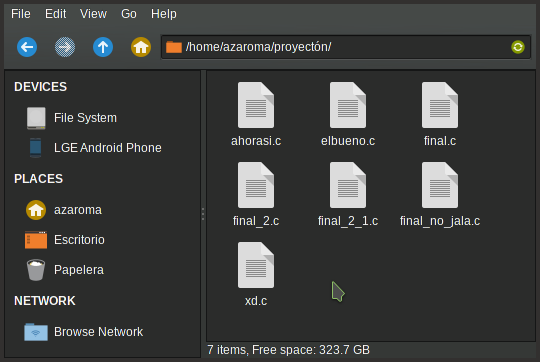
\includegraphics[width=\textwidth]{version}
      \caption{Control de versiones antiguo}
    \end{figure}
  \end{columns}
\end{frame}

\begin{frame}
\frametitle{¿Por qué Git?}
\begin{figure}
  \centering
  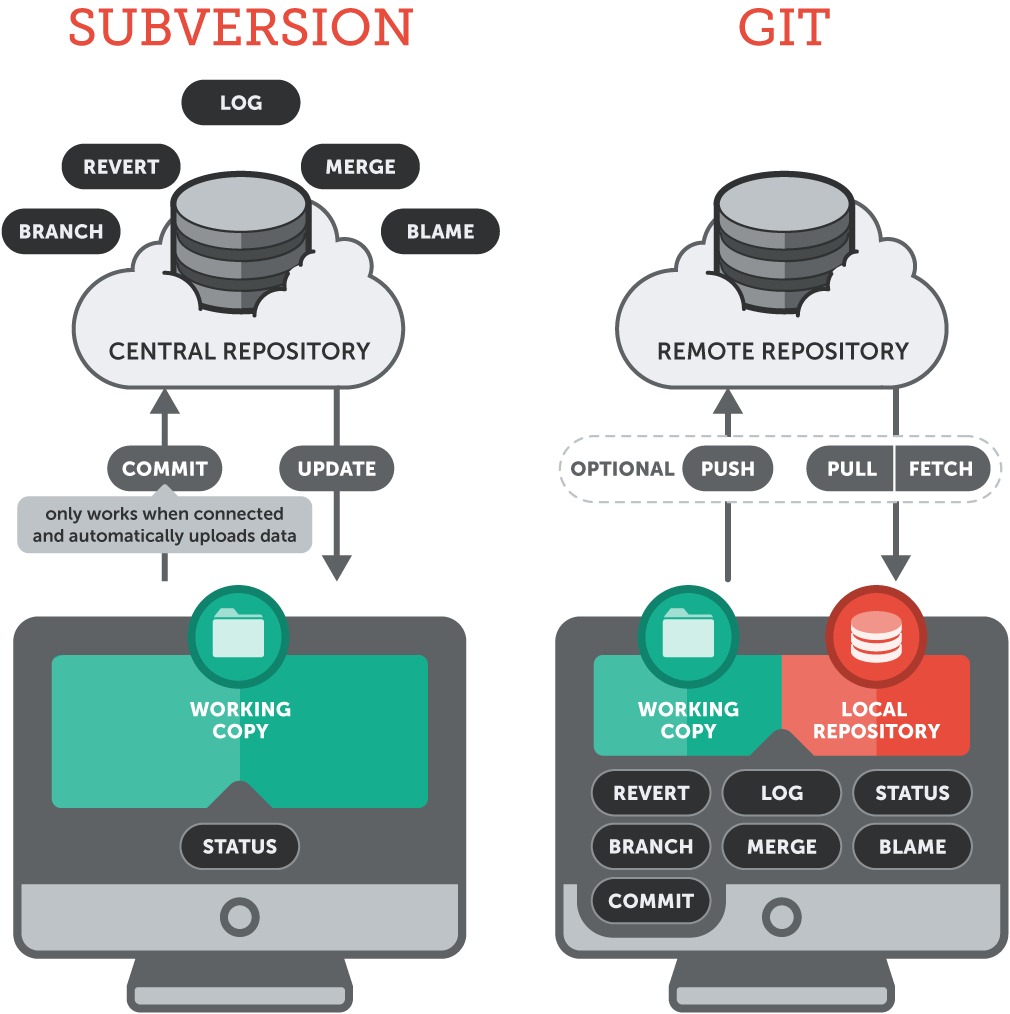
\includegraphics[scale=0.2]{centralizado-vs-distribuido}
  \caption{Diferencias entre un sistema de control de versiones distribuido y uno centralizado}
\end{figure}
\end{frame}

\begin{frame}
\frametitle{Repositorio}
Estructura de datos que almacena metadatos y/o un sistema de archivos.

\vspace{2em}

\colorbox{purple}{\color{white}{\lstinline|git init|}} convierte el directorio actual en un repositorio.

\vspace{1em}

\colorbox{purple}{\color{white}{\lstinline°git clone <http|ftp|ssh>°}} crea una copia local de un repositorio remoto.
\end{frame}

\begin{frame}
  \begin{center}
    \resizebox{\textwidth}{!}{\FiraTitle \color{green}{git status}}
    \resizebox{0.7\textwidth}{!}{\FiraTitle \color{purple}{git log}}
  \end{center}
\end{frame}

\begin{frame}
  \frametitle{git add}
  \begin{figure}
    \centering
    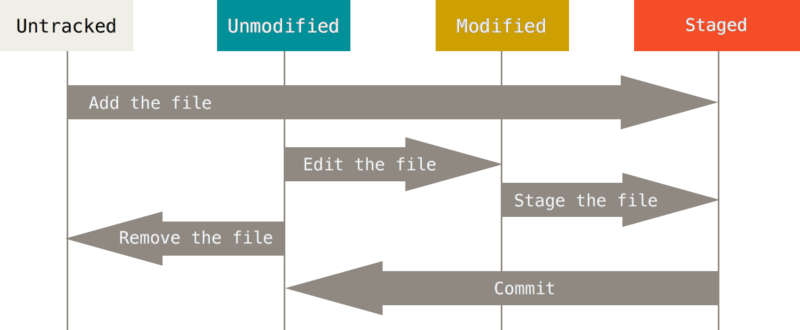
\includegraphics[width=\textwidth]{ciclo}
    \caption{Ciclo de vida de los archivos en git}
  \end{figure}
\end{frame}

\begin{frame}
  \begin{center}
    \resizebox{\textwidth}{!}{\FiraTitle \color{green}{.gitignore}}
    \vspace{1em}
    
    {\FiraTitle Indica cuales archivos debe ignorar git}
    \vspace{1em}
  \end{center}
  {\FiraTitle \color{purple}{Glob patterns:}}
  \begin{itemize}
  \item \textbf{* :} Cero o más caracteres
  \item \textbf{[abc] :} Cualquiera de los caracteres dentro de los corchetes
  \item \textbf{? :} Un sólo caracter
  \item \textbf{[0-9] :} Rango
  \end{itemize}
\end{frame}

\begin{frame}
  \resizebox{0.7\textwidth}{!}{\FiraTitle \color{purple}{git commit}}
  \vspace{2em}

  \begin{columns}
    \column{0.8\textwidth}
    {\FiraTitle Mejores prácticas}
    \begin{enumerate}
    \item Separar el tema del cuerpo del mensaje
    \item Tema de 50 caracteres
    \item El tema inicia con mayúsculas
    \item El tema no lleva punto
    \item Usar verbos imperativos
    \item Líneas de 72 caracteres en el cuerpo
    \item El cuerpo explica el qué y el por qué
    \end{enumerate}

    \column{0.2\textwidth}
    \begin{figure}
      \centering
      
\includegraphics[width=\textwidth]{camera}
    \end{figure}
  \end{columns}
\end{frame}

\begin{frame}
  \begin{center}
    \resizebox{0.7\textwidth}{!}{\FiraTitle \color{green}{Branching}}
  \end{center}
  \begin{figure}
    \centering
    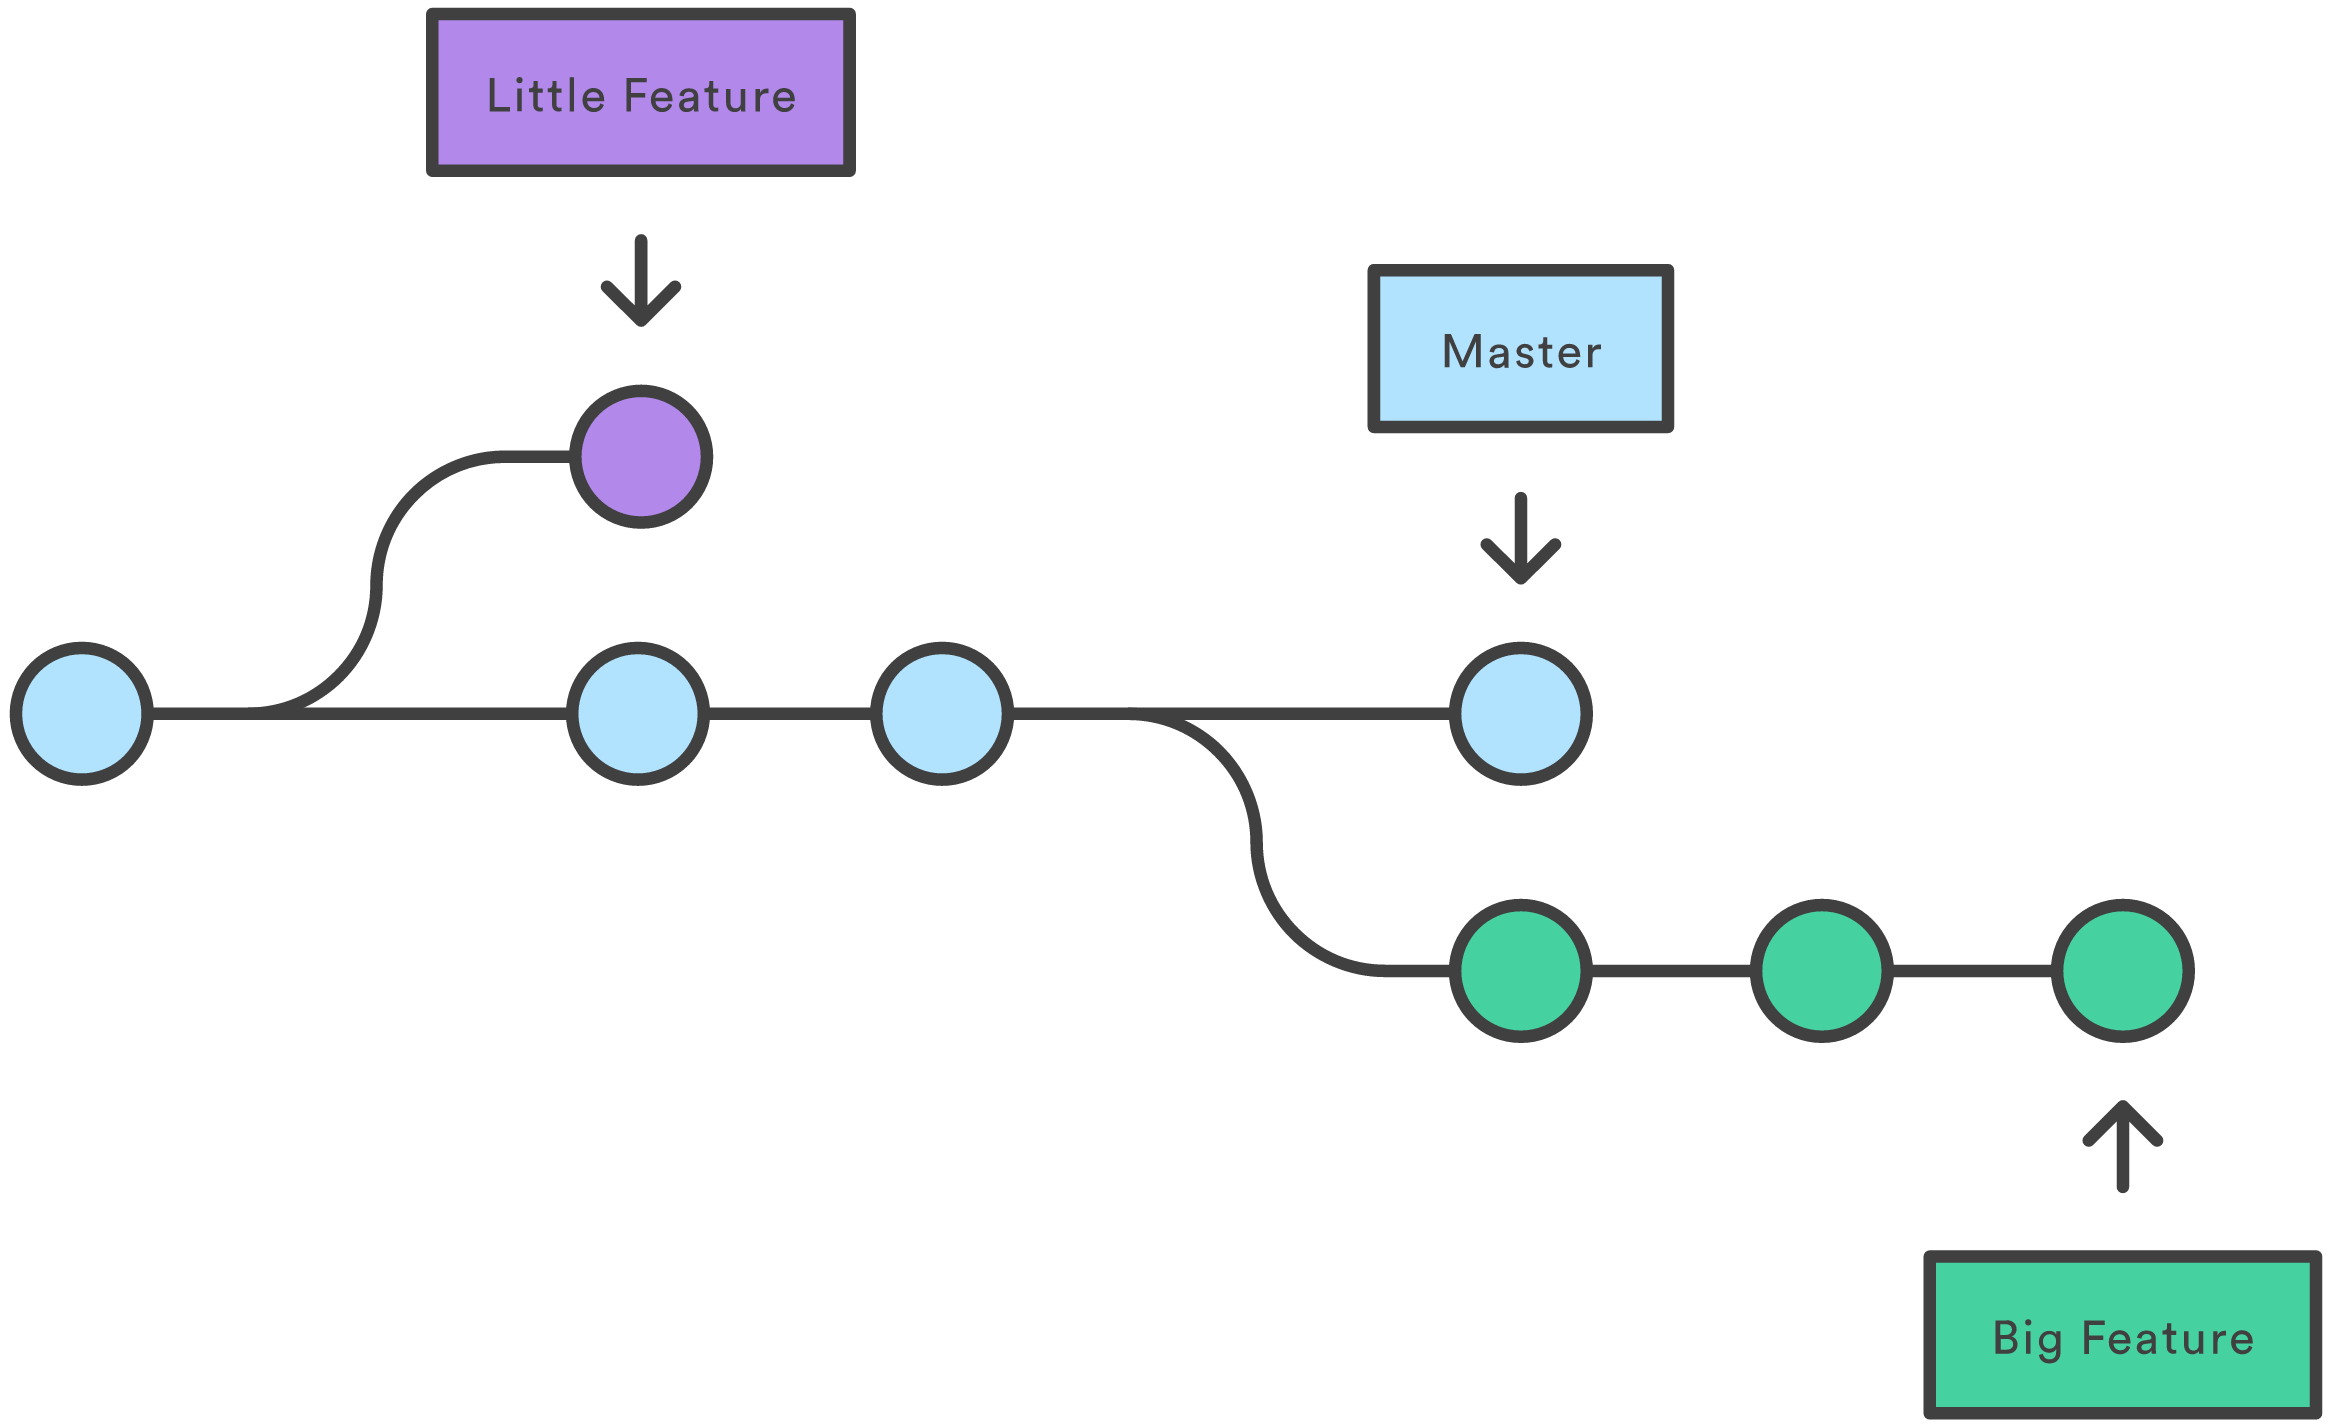
\includegraphics[width=0.9\textwidth]{ramas}
  \end{figure}
\end{frame}

\begin{frame}
  \begin{center}
    \resizebox{0.6\textwidth}{!}{\FiraTitle \color{purple}{Merging}}
  \end{center}
  \begin{figure}
    \centering
    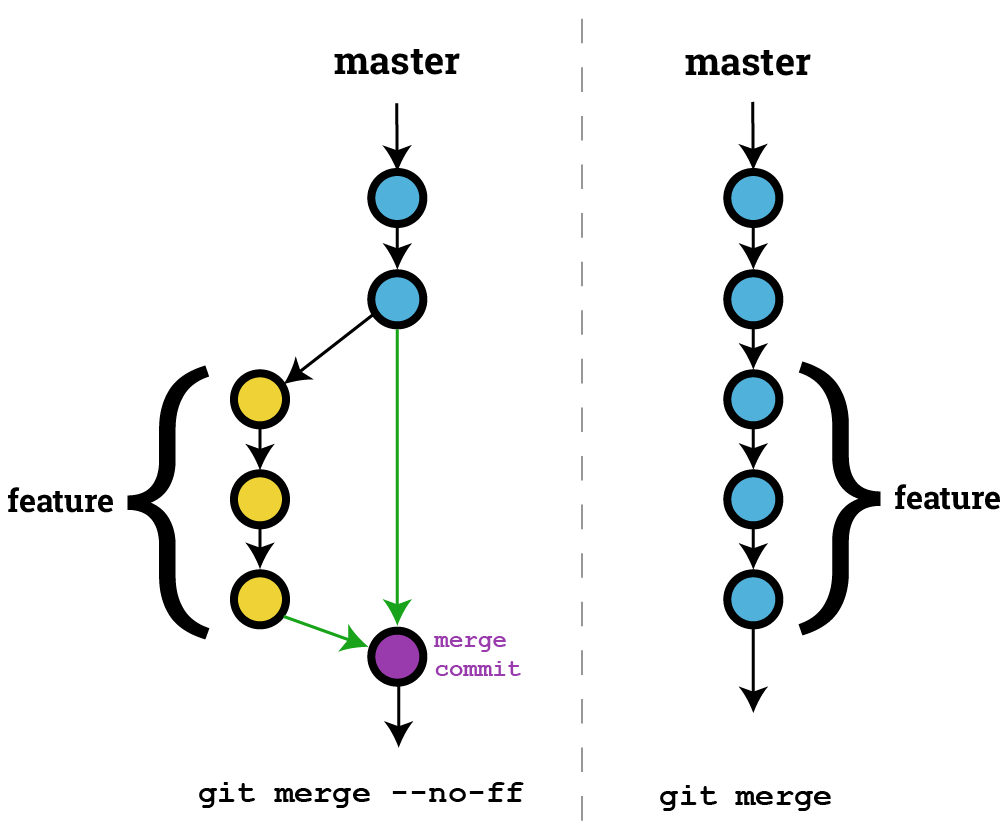
\includegraphics[height=0.7\textheight]{fusion}
  \end{figure}
\end{frame}

\begin{frame}
\frametitle{Github}
\end{frame}

\begin{frame}
\frametitle{Remote}
\end{frame}

\begin{frame}
\frametitle{Clone}
\end{frame}

\begin{frame}
\frametitle{Pull}
\end{frame}

\begin{frame}
\frametitle{Push}
\end{frame}

\begin{frame}
\frametitle{Flujo de trabajo}
\end{frame}

\begin{frame}
\frametitle{Observaciones finales}
\end{frame}

\begin{frame}
  \frametitle{Referencias}
\end{frame}

\end{document}
